
\section{\textit{PageRank}}

  %\subsection{Definição}
  \label{sec:dpr}

  O conceito de \textit{PageRank} é conhecido como um método de determinar o ranking das páginas web para os motores de busca. 
  Este algoritmo tem como base um algoritmo de \textit{random walk} em que um walker num determinado vértice $u$ salta para um vértice adjacente $v$ com uma probabilidade $d_g(u)$.
  
  \subsection{Algoritmo de \textit{PageRank}}
  Para calcular o \textit{PageRank} de um grafo G=(V,E) em que a sua matriz de adjacência A$_{u,v}$ = $w(u,v)$\footnote{$w(u,v)$ é a função que indica o peso do arco $(u,v)$.} e com uma matriz diagonal D em que D$_{u,u}$=$d_G(u)$\footnote{$d_G(u)$ pode indicar o degree de um vértice no caso de o grafo não ser direccionado ou o out-degree caso este seja direccionado.}, pode ser utilizada a seguinte formula:
  
\[ P_\alpha(n) = \left\{
  \begin{array}{l l}
    \alpha P_0+(1-\alpha)P_\alpha(n-1)D^{{-}1}A & \quad \text{, se } n>0   \\
    P_0 & \quad \text{, se }n=0 
  \end{array} \right.\]
  
  A formula apresentada tem um conjunto de parâmetros que são utilizados para calcular o \textit{PageRank}. O P$_0$ indica a probabilidade inicial de um vértice, seguindo normalmente uma distribuição normal (1/$|V|$). O $\alpha$ é denominado de \textit{jumping factor} e garante que um navegador não chegue a um vértice que não tenha ligação com um outro. A matriz $M=D^{{-}1}A$ representa a matriz de transição de uma \textit{random walk}.
  
  \paragraph{Exemplo}  
  No processamento sequencial do \textit{Page Rank}, podendo ter mas matrizes necessárias à computação em memória, basta aplicar a forma apresentada na Definição do algoritmo até se chegar a um valor de convergência.
   
  \begin{figure}[h]
    \centering
    \caption{Grafo de exemplo.}
    \scalebox{0.5}{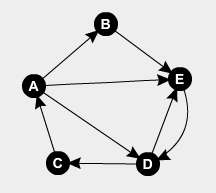
\includegraphics{graph_example.png}}%\\
    \label{graph}
  \end{figure}

  Para um grafo direccionado (Figura \ref{graph}) com todas os arcos com peso de 1, pode-se calcular o \textit{PageRank} da seguinte forma:\\[0.25cm]
 
  Neste exemplo vai-se usar $\alpha=0.85$.
 
  Sabendo que a matriz de adjacência do grafo da Figura \ref{graph} é 
  $A=	\begin{bmatrix}
	  0 & 1 & 0 & 1 & 1 \\
	  0 & 0 & 0 & 0 & 1 \\
	  1 & 0 & 0 & 0 & 0 \\
	  0 & 0 & 1 & 0 & 1 \\
	  0 & 0 & 0 & 1 & 0 \\
	\end{bmatrix}$\\[0.25cm]
   e que a matriz $D^{{-}1}= \begin{bmatrix}
				1/3 & 0 & 0 & 0 & 0 \\
				0 & 1 & 0 & 0 & 0 \\
				0 & 0 & 1 & 0 & 0 \\
				0 & 0 & 0 & 1/2 & 0 \\
				0 & 0 & 0 & 0 & 1 \\
			      \end{bmatrix}$.
  \\[0.25cm]
  A matriz M (matriz de \textit{random walk}) é dada pela seguinte expressão:
  
  $M=AD^{{-}1}= \begin{bmatrix}
		0 & 1/3 & 0   & 1/3 & 1/3 \\
		0 & 0   & 0   & 0   & 1   \\
		1 & 0   & 0   & 0   & 0   \\
		0 & 0   & 1/2 & 0   & 1/2 \\
		0 & 0   & 0   & 1   & 0   \\
	      \end{bmatrix}$
  \\[0.25cm]
  \begin{bf}
    Para n=0:
  \end{bf}
  
  $P_\alpha(0) = P_0 = \begin{bmatrix} 1/5 & 1/5 & 1/5 & 1/5 & 1/5 \end{bmatrix}$ (seguindo uma distribuição uniforme)
  \\[0.25cm]
  \begin{bf}
    Para  n=1:
  \end{bf}
  
  $P_\alpha(1) = \alpha P_0 + (1-\alpha)P_\alpha(0)M = \\[0.25cm]
  =0.85\begin{bmatrix} 1/5 & 1/5 & 1/5 & 1/5 & 1/5 \end{bmatrix} + 0.15 \begin{bmatrix} 1/5 & 1/5 & 1/5 & 1/5 & 1/5 \end{bmatrix} \begin{bmatrix}
		0 & 1/3 & 0   & 1/3 & 1/3 \\
		0 & 0   & 0   & 0   & 1   \\
		1 & 0   & 0   & 0   & 0   \\
		0 & 0   & 1/2 & 0   & 1/2 \\
		0 & 0   & 0   & 1   & 0   \\
	      \end{bmatrix}=\\[0.25cm]
  =\begin{bmatrix} 17/100 & 17/100 & 17/100 & 17/100 & 17/100 \end{bmatrix} + \begin{bmatrix} 3/100 & 1/100 & 3/200 & 1/25 & 11/200 \end{bmatrix}=\\[0.25cm]
  =\begin{bmatrix} 1/5 & 9/50 & 37/200 & 21/100 & 9/40 \end{bmatrix}
$
  \\[0.25cm]
  Pode-se repetir este processo até que $P_\alpha(n) \approx P_\alpha(n-1)$, isto é,
  até ter chegado a um valor perto do seu valor de convergência.
  
  \subsection{Algoritmo de \textit{PageRank} Distribuído}
  \label{sec:prdistributed}

  Para redes de grandes dimensões é difícil de manter todos o seu estado em memória, daí da necessidade de utilizar sistemas distribuídos. 

  Em ambientes distribuídos é difícil se ter acesso a todo o estado do grafo daí que haja algumas alterações à forma como se obtém o \textit{rank} do vértice. Estas alterações vêem do facto de se calcular em cada vértice um \textit{rank} intermédio e enviar informação sobre o seu \textit{rank} aos vértices adjacentes
  O \textit{rank} de um vértice é calculado sabendo a contribuição dos vértices adjacentes, podendo ser calculado da seguinte forma:
  
  \begin{center}
    \begin{equation}
      \label{eq:prrankdistributed}
       P_v = (1-\alpha) * C(N_g(v)) + \alpha/ow(v)
    \end{equation}
    Sendo $C(N_g(v))$ o somatório das contribuições dos vértices adjacentes, $ow(v)$ o somatório dos pesos das $out-edges$ e $\alpha$ o $jumping factor$ descrito na secção \ref{sec:dpr}.
  \end{center}    
  
  A contribuição de um vértice v para os seus adjacente é calculada da seguinte maneira:
 
  \begin{center}
    \begin{equation}
      \label{eq:prcontributiondistributed}
       C_v=R_v/ow(v)
    \end{equation}
    Sendo $R_v$ o \textit{rank} que o vértice tem de momento.
  \end{center}    
  
  Numa plataforma que segue o modelo BSP o algoritmo pode ser descrito para cada vértice da seguinte maneira:
  \begin{algorithm}
    \caption{\textit{PageRank} Distribuído}\label{alg:prdistributed}
    \begin{enumerate}
      \item No primeiro \textit{superstep}, iniciar o valor de cada vértice com a sua probabilidade inicial.
      \item Enviar para os vértices adjacentes a sua contribuição.
      \item Num \textit{superstep} diferente do primeiro, calcular o rank do vértice.
      \item Repetir o algoritmo a partir do item 2 durante um número pré-configurado de iterações.
    \end{enumerate}
  \end{algorithm}
  
\section{\textit{heat-kernel}}

  %\subsection{Definição}
  \label{sec:heatkerneldefinition}
  
    Tal como o \textit{PageRank}, o \textit{heat-kernel}, é também baseado numa \textit{random walk}. 
    É  definida a matriz $L=I-M$, sendo M a matriz de transição de uma \textit{random walk} que tabém é usada no \textit{PageRank}.
    
    O \textit{heat-kernel} pode ser definido pela seguinte formula:\\
    $P_t(n)=P_0(I+\frac{-t}{n}L)^n$
	
  \subsection{Algoritmo de \textit{heat-kernel}}
  O que diferencia o \textit{heat-kernel} do \textit{PageRank} é  facto deste satisfazer a equação de calor. A constante $t$ que aparece na formula podem assumir valores superiores ou iguais a 0 e representa a condutividade térmica. Quanto mais alto esta constante for, mais rápida será a propagação do calor.  
    
  \paragraph{Exemplo}   
  Para o grafo apresentado na Figura \ref{graph} pode-se calcular o \textit{heat-kernel} da seguinte maneira (sendo as matrizes $A$ e $D^{{-}1}$ iguais no exemplo apresentado sobre o \textit{PageRank} ): \\[0.25cm]
  Vai-se considerar para este exemplo $t=1/2$. \\[0.25cm]
  $L = I_5 - M = \begin{bmatrix} 
		    1 & -1/3 & 0 & -1/3 & -1/3 \\
		    0 & 1 & 0 & 0 & -1 \\
		    -1 & 0 & 1 & 0 & 0\\
		    0 & 0 & -1/2 & 1 & -1/2\\
		    0 & 0 & 0 & -1 & 1\\
		 \end{bmatrix}$
  \\[0.25cm]
  \begin{bf}
    Para n=0:
  \end{bf}
  
  $P_t(0) = P_0 = \begin{bmatrix} 1/5 & 1/5 & 1/5 & 1/5 & 1/5 \end{bmatrix}$
  \\[0.25cm]
  \begin{bf}
    Para n=1:
  \end{bf}
  
  $P_t(n)=P_0(I_5+\frac{-1/2}{1}L)^1=\\[0.25cm]
  =\begin{bmatrix} 1/5 & 1/5 & 1/5 & 1/5 & 1/5 \end{bmatrix} (
		\begin{bmatrix} 
		    1 & 0 & 0 & 0 & 0\\
		    0 & 1 & 0 & 0 & 0\\
		    0 & 0 & 1 & 0 & 0\\
		    0 & 0 & 0 & 1 & 0\\
		    0 & 0 & 0 & 0 & 1\\
		 \end{bmatrix} +
		 \begin{bmatrix} 
		    1/2 & -1/6 & 0 & -1/6 & -1/6 \\
		    0 & 1/2 & 0 & 0 & -1/2 \\
		    -1/2 & 0 & 1/2 & 0 & 0\\
		    0 & 0 & -1/4 & 1/2 & -1/4\\
		    0 & 0 & 0 & -1/2 & 1/2\\
		 \end{bmatrix}) = \\[0.25cm]
  = \begin{bmatrix} 1/5 & 1/5 & 1/5 & 1/5 & 1/5 \end{bmatrix}
    \begin{bmatrix} 
      3/2 & -1/6 & 0 & -1/6 & -1/6 \\
      0 & 3/2 & 0 & 0 & -1/2 \\
      -1/2 & 0 & 3/2 & 0 & 0\\
      0 & 0 & -1/4 & 3/2 & -1/4\\
      0 & 0 & 0 & -1/2 & 3/2\\
    \end{bmatrix} = \\[0.25cm]
  = \begin{bmatrix} 1/5 & 4/15 & 1/4 & 1/6 & 7/60 \end{bmatrix}$\\[0.25cm]
  
  Tal como o \textit{PageRank}, faz-se este processo até que $P_t(n) \approx P_t(n-1)$.

  \subsection{Algoritmo de \textit{heat-kernel} Distribuído}
  
  O \textit{heat-kernel} distribuído tal como o \textit{PageRank} distribuído(secção \ref{sec:prdistributed}) passa por se calcular um \textit{rank} intermédio e enviar a sua contribuição para os vértices adjacentes.
  
  \begin{center}
    \begin{equation}
      \label{eq:heatkerneldistributedrank}
       P_v = P_v + C(N_g(v)) + P_i * (1 - t/N)
    \end{equation}
    Sendo $C(N_g(v))$ o somatório das contribuições dos vértices adjacentes, $P_i$  o valor inicial do vértice, $t$ a constante de condutividade térmica (referenciado na secção \ref{sec:heatkerneldefinition} e $N$ o total de \textit{iterações}).
  \end{center}    
  
  A contribuição de um vértice $v_1$ para um vértice $v_2$ é calculada da seguinte maneira:
  
  \begin{center}
    \begin{equation}
      \label{eq:heatkerneldistributedcontribution}
       Cv_1=P_i * t / N * w(v_1,v_2)/ow(v_1))
    \end{equation}
    Sendo $w(v_1,v_2)$ o peso da \textit{edge} entre $v_1$ e $v_2$ e $ow(v_1)$ o somatório dos pesos das $out-edges$.
  \end{center}  
  
  O algoritmo do \textit{heat-kernel} pode ser descrito da mesma forma que o algoritmo do \textit{PageRank}(\textit{Algorithm} \ref{alg:prdistributed} na secção \ref{sec:prdistributed}).
  